\documentclass[12pt]{article}
\usepackage[english]{babel}
\usepackage[utf8]{inputenc}
\usepackage{amsmath, amssymb, amsthm}
\usepackage{graphicx}
\usepackage{hyperref}
\usepackage{geometry}
\usepackage{xcolor}
\usepackage{tikz}

\setlength{\topmargin}{0pt}
\setlength{\headsep}{0pt}
\textheight = 600pt

\title{Graph Theory \\ Homework 2}
\author{Ben Kallus and Maddy LaPoint}
\date{Due Wednesday, February 10}

\begin{document}
\pagecolor{black}
\color{white}
\maketitle

\noindent{\bf 1.16}
\begin{proof}
    Let $P = (u = v_0, v_1, \hdots, v_k = v), k \geq 1$, be a $u-v$ geodesic in a connected graph $G$.
    We claim that $d(u,v_i)=i$ for each integer $i$ with $1 \leq i \leq k$.
    Suppose, toward a contradiction, that there exists an integer $i$ with $1 \leq i \leq k$ such that $d(u,v_i) \neq i$.
    Then $d(u,v_i) < i$, since $(u = v_0 \hdots, v_i)$ is a $u-v_i$ walk of length $i$.
    Therefore, there exists a $u-v_i$ path $Q$ with length $j < i$.
    Define $R$ to be the walk obtained by first following $Q$, and then following $(v_i, \hdots, v_k)$.
    The length of $R$ is therefore $k - i + j$.
    Thus, since $j$ is less than $i$, the length of $R$ is less than $k$.
    Thus, $d(u,v) < k$.
    However, since $P$ is a $u-v$ geodesic of length $k$, $d(u,v)=k$.
    Thus, $d(u,v_i)=i$ for each integer $i$ with $1 \leq i \leq k$.
\end{proof}

\bigskip
\noindent{\bf 1.15}
\begin{center}
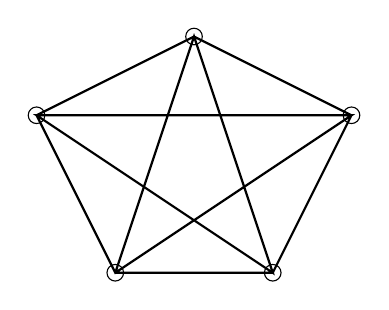
\begin{tikzpicture}
    \draw[fill=white] (1,0) circle (3pt);
    \draw[fill=white] (3,0) circle (3pt);
    \draw[fill=white] (4,2) circle (3pt);
    \draw[fill=white] (2,3) circle (3pt);
    \draw[fill=white] (0,2) circle (3pt);

    \draw[thick] (1,0) -- (3,0) -- (4,2) -- (2,3) -- (0,2) -- (1,0) -- (4,2) -- (0,2) -- (3,0) -- (2,3) -- (1,0);
\end{tikzpicture}
\end{center}

    % Should this be more formal?
    Suppose there were another graph $G$ of order 5 with odd distances between every two distinct vertices.
    Then, since $G$ is not the complete graph of order 5, there exist two vertices $u,v \in V(G)$ with $d(u,v) \in \{3,5\}$.
    Then, there exists a $u-v$ geodesic $P = (u=v_0, v_1, v_2, \hdots, v_{d(u,v)}=v)$ with length at least 3.
    By the result of exercise 1.16, $d(u,v_2) = 2$.
    Thus, the complete graph of order 5 is the only graph of order 5 with odd distances between every two distinct vertices.

\newpage
\noindent{\bf 1.17}

\noindent{\bf (a)}
\begin{proof}
    Let $P=(p_0, \hdots, p_k)$ and $Q=(p_0, \hdots, p_k)$ be two paths of length $k$ in a connected graph $G$ with diameter $k$.
    We claim that $P$ and $Q$ have at least one vertex in common.
    Suppose, toward a contradiction, that $P$ and $Q$ have no vertex in common.
    Since $G$ is connected, there exists a $u-v$ path $R$ with $u \in P$ and $v \in Q$.
    Define $R'$ to be the shortest subsequence of $R$ that begins with an element of $P$ and ends with an element of $Q$.
    Since $P$ and $Q$ have no vertex in common, the length of $R'$ is at least 1.
    Let $p_i$ and $q_j$ be the first and last elements of $R'$, respectively.
    % I don't feel like writing it out formally, but here 's the rest of the proof:
    % Make a new path starting at either p_0 or p_k, which ever is further from p_i, traveling along P (either backwards or forwards depending on startpoint), passing through R', and then finishing at either q_0 or q_k, whichever is further from q_j, traveling along Q (either backwards or forwards). This is a path, since P and Q are independent paths, so they don't share any vertices, and R' cant cause it to not be a path because it is the shortest path between P and Q. If it had an extra element of either P or Q, then it could be shortened. This new path is at least length k+1, since each of the parts along P and Q is at least length ceil(k/2), and R' is at least length 1. Thus, the new path has length 2 * ceil(k/2) + 1 >= 2 * k/2 + 1 = k + 1. So we're at a contradiction.
\end{proof}

\medskip
\noindent{\bf (b)}
\begin{proof}
    Let $G$ be a connected graph of diameter $k$.
    We claim that two geodesics of length $k$ in $G$ do not necessarily have a vertex in common.
    Consider the complete graph of order 4, with vertices $\{c_1, c_2, c_3, c_4\}$.
    Since there exists an edge between all pairs of distinct vertices in this graph, it has diameter 1.
    Observe that the edges $c_1c_2$ and $c_3c_4$ are geodesics of length 1 that do not share a vertex.
    Thus, two geodesics of length $k$ in $G$ do not necessarily have a vertex in common.
\end{proof}

\bigskip
\noindent{\bf 1.19}
% I think it's always safe to remove an endpoint of a longest path in the graph. Removing this vertex can't disconnect the graph because if it did, then that would mean that the rest of the longest path is not connected to the vertices past the endpoint, so we could make the path longer by connecting the endpoint to one of the vertices in the area that it would disconnect.
% You can iterate this process $|V| - 1$ times, so the answer is yes.

\bigskip
\noindent{\bf 1.21}

    % Draw 3 4-length lines, 2 squares, and 1 box with diagonals

\bigskip
\noindent{\bf 1.22}

    % case 1: $uv \notin G$. Thus, $uv \in \overline G$, so $d_{\overline G}(u,v)=1$. & might need to account for u=v depending on wording
    % case 2.1: $uv \in G$. Since $G$ is disconnected, it has at least 2 components. Since $uv \in G$, $u,v$ are in the same component in $G$. Let $w$ be a vertex in another component in $G$. Then, $uw, wv \in \overline G$. Thus, $d_{\overline G}(u,v) \leq 2$.
    % QED

\bigskip
\noindent{\bf 1.24}

    % $G_1$ is bipartite, $G_2$ is not (because of odd cycle theorem)
    % Drawing is trivial, but annoying.

\end{document}